% ex: ts=2 sw=2 sts=2 et filetype=tex
% SPDX-License-Identifier: CC-BY-SA-4.0

\documentclass[12pt,addpoints]{exam}

\usepackage[utf8]{inputenc}
\usepackage[T1]{fontenc}
%\usepackage[spanish]{babel}
\usepackage[letterpaper]{geometry}

\pagestyle{headandfoot}
\headrule
\header{Física II}{Examen}{CBTIS 246}
\footer{}{Página \thepage\ de \numpages}{}

\pointpoints{punto}{puntos}
\renewcommand{\solutiontitle}{\textbf{Solución: }}

\printanswers

\begin{document}
%\begin{center}
%\fbox{\fbox{\parbox{5.5in}{\centering
%Lee con atención cada pregunta y responde en
%el espacio ubicado en la parte izquierda.
%}}}
%\end{center}
%
%\vspace{5mm}

Nombre:\enspace\hrulefill

\vspace{5mm}

Grupo:\enspace\hrulefill
\enspace{}Grado:\enspace\hrulefill
\enspace{}Fecha:\enspace\hrulefill

\begin{questions}

% ex: ts=2 sw=2 sts=2 et filetype=tex
% SPDX-License-Identifier: CC-BY-SA-4.0

\question Es cada uno de los elementos que componen la población:

  \begin{oneparchoices}
    \CorrectChoice Individuo
    \choice Dato
    \choice Entrevista
  \end{oneparchoices}

% ex: ts=2 sw=2 sts=2 et filetype=tex
% SPDX-License-Identifier: CC-BY-SA-4.0

\question Los \fillin\ se caracterizan porque las partículas que
los componen están muy cercanas entre sí, y en posiciones más o menos fijas

  \begin{oneparchoices}
    \choice Líquidos
    \choice Gaseosos
    \CorrectChoice Sólidos
    \choice Todos
  \end{oneparchoices}
  \answerline[C]

% ex: ts=2 sw=2 sts=2 et filetype=tex
% SPDX-License-Identifier: CC-BY-SA-4.0

\question Como se llaman los lados que forman el ángulo recto en un
          triángulo rectángulo.

  \begin{oneparchoices}
    \choice Lado de 90 grados
    \choice Lado recto
    \choice Hipotenusa
    \CorrectChoice Cateto
  \end{oneparchoices}
  \answerline[D]

% ex: ts=2 sw=2 sts=2 et filetype=tex
% SPDX-License-Identifier: CC-BY-SA-4.0

\question \[ \frac{8}{4} + \frac{9}{4} = \frac{\hspace{2cm}}{\hspace{2cm}} 
             \hspace{2cm}
             \frac{5}{2} + \frac{4}{3} = \frac{\hspace{2cm}}{\hspace{2cm}}
          \]


% ex: ts=2 sw=2 sts=2 et filetype=tex
% SPDX-License-Identifier: CC-BY-SA-4.0

\question \[ \frac{7}{5} - \frac{5}{5} = \frac{\hspace{2cm}}{\hspace{2cm}}
             \hspace{2cm}
             \frac{2}{2} - \frac{1}{4} = \frac{\hspace{2cm}}{\hspace{2cm}}
          \]

% ex: ts=2 sw=2 sts=2 et filetype=tex
% SPDX-License-Identifier: CC-BY-SA-4.0

\question $x^2 - 25$


% ex: ts=2 sw=2 sts=2 et filetype=tex
% SPDX-License-Identifier: CC-BY-SA-4.0

\question $a^2 - 64$


% ex: ts=2 sw=2 sts=2 et filetype=tex
% SPDX-License-Identifier: CC-BY-SA-4.0

\question Una urna contiene canicas de colores: 8 Azules, 12 moradas,
4 negras y 16 rojas. Completa los siguientes espacios de la tabla y
determina cuál es la probabiliad de que al hacer una extracción esta
sea de color ... 

  \begin{tabular}{|l|c|c|l|l|l|}
    \hline
    \textbf{Evento} &  \textbf{Casos} & \textbf{Casos} &
    \textbf{Probabilidad} & \textbf{Decimal} &  \textbf{Porcentaje} \\
     &  \textbf{favorables} & \textbf{posibles} & & & \\
    \hline
    Azul & & & & & \\
    \hline
    Morado & & & & & \\
    \hline
    Negro & & & & & \\
    \hline
    Rojo & & & & & \\
    \hline
    \textbf{Suma} & & \textbf{Suma} & & & \\
    \hline
  \end{tabular}

% ex: ts=2 sw=2 sts=2 et filetype=tex
% SPDX-License-Identifier: CC-BY-SA-4.0

\question 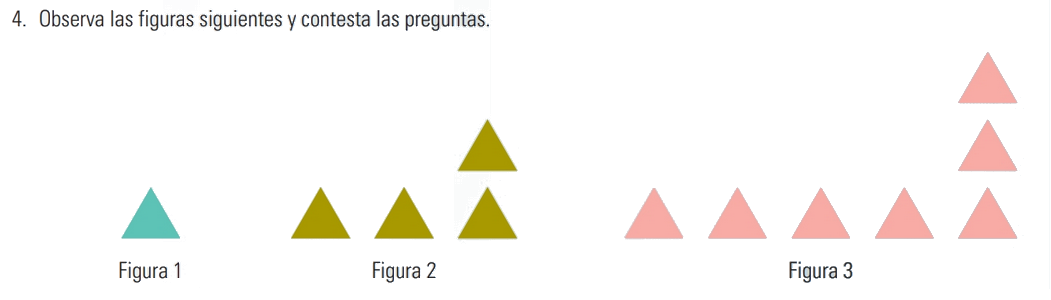
\includegraphics[scale=0.4]{p/i021.png} 
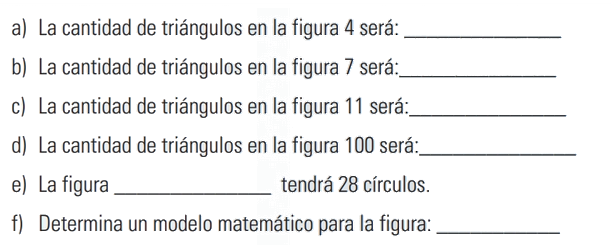
\includegraphics[scale=0.5]{p/i031.png} 

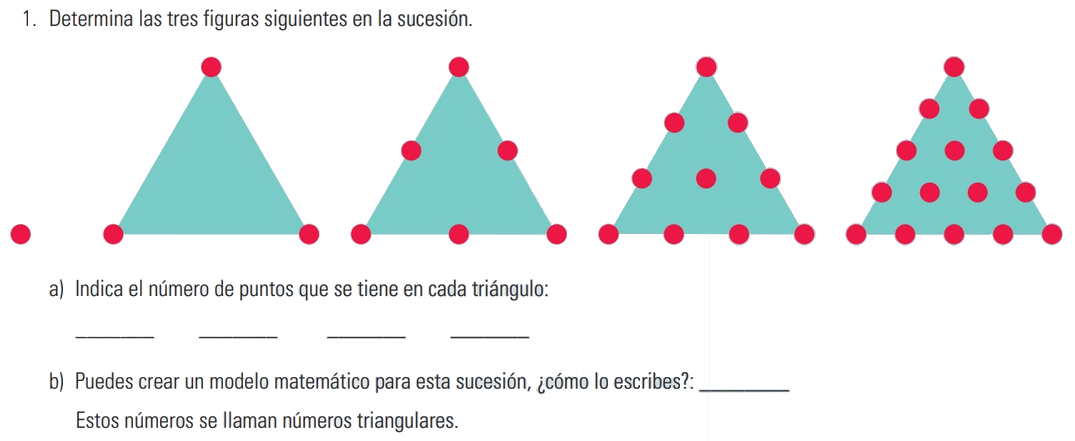
\includegraphics[scale=0.4]{p/i041.png} 
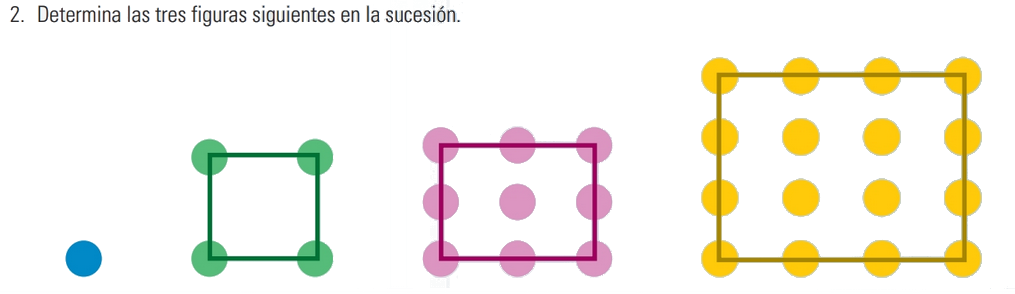
\includegraphics[scale=0.4]{p/i051.png} 

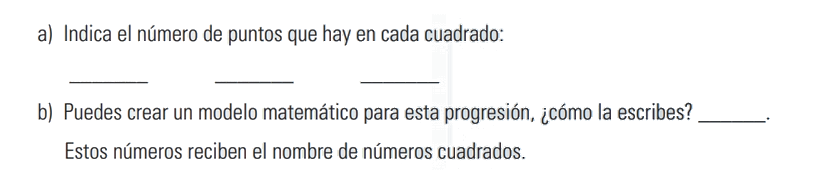
\includegraphics[scale=0.4]{p/i061.png} 


\end{questions}

\end{document}
